\chapter{The n2EDM experiment}
\label{chapter:experiment}

Knowledge is power and our knowledge of the physical property that can be measured to show the violation of the \textit{CP}-symmetry is an important first step in solving the riddle of the baryogenesis. Now we just need to get our hands dirty with some experimental data. It will be obtained over the course of the n2EDM experiment currently being built at PSI (Paul Scherrer Institute, Villigen, Switzerland).

\textit{What will be measured?} Electric dipole moment of the neutron. The neutrons were chosen for the following reasons:
\begin{itemize}
	\item They are electrically neutral\footnote{Which is quite important for an experiment based in Switzerland}, which means that they would not be dragged by the electric field $\vec{E}$
	\item There are nuclear reactions that allow to produce them efficiently, like fission or spallation (which is already available in PSI and will be used)
	\item They can be cooled down to become UCNs (ultracold neutrons)
\end{itemize}

\textit{What are ultracold neutrons and why do we like them?} We call \cite{Fermi1936} a neutron ultracold when it has a kinetic energy $E_{kin} \leq 300\ \text{neV}$. Such low energy brings the following experimental benefits:
\begin{itemize}
	\item Ease of collection, since the neutrons would behave similar to ping-pong balls, bouncing from the surface of a neutron vessel.
	\item Possibility to store \cite{Zeldovich1959} the neutrons up to their lifetime of $\approx 886\ \text{s}$ \cite{Tanabashi2018}.
	\item Weakening of a so-called $\vec{v} \times \vec{E}$ effect \cite{Pendlebury2004}, which arises from the coupling of a particle spin $\vec{I}$ itself with an electric field $\vec{E}$. This would bring the effective Hamiltonian closer to one mentioned in Eq. \ref{eq:neutron_hamiltonian}.
\end{itemize}

\textit{What precision do we expect?} By using only the Standard Model it is possible to get an estimation \cite{Khriplovich1982} of the neutron EDM at the following level:
\begin{equation}
	d_n \approx 2 \cdot 10^{-32}\ e \cdot \text{cm}
\end{equation}

The \textbf{n2EDM} experiment is conceptually following the footsteps of the results obtained by the \textbf{nEDM} collaboration. By analysing the data obtained at ILL, Grenoble it was possible to achieve \cite{Pendlebury2015} an impressive record of $d_n$ precision:
\begin{equation}
	\left| d_n \right| < 3.6 \cdot 10^{-26}\ e \cdot \text{cm (95\% CL)}.
\end{equation}

This leaves us with 6 more orders of magnitude to go. The n2EDM experiment aims to cut this number to five, improving \cite{Abel2018} the precision tenfold.

\textit{What method will be used?} Same as in the original nEDM experiment, Ramsey method of the time separated oscillating fields.%
\begin{figure}[h]
	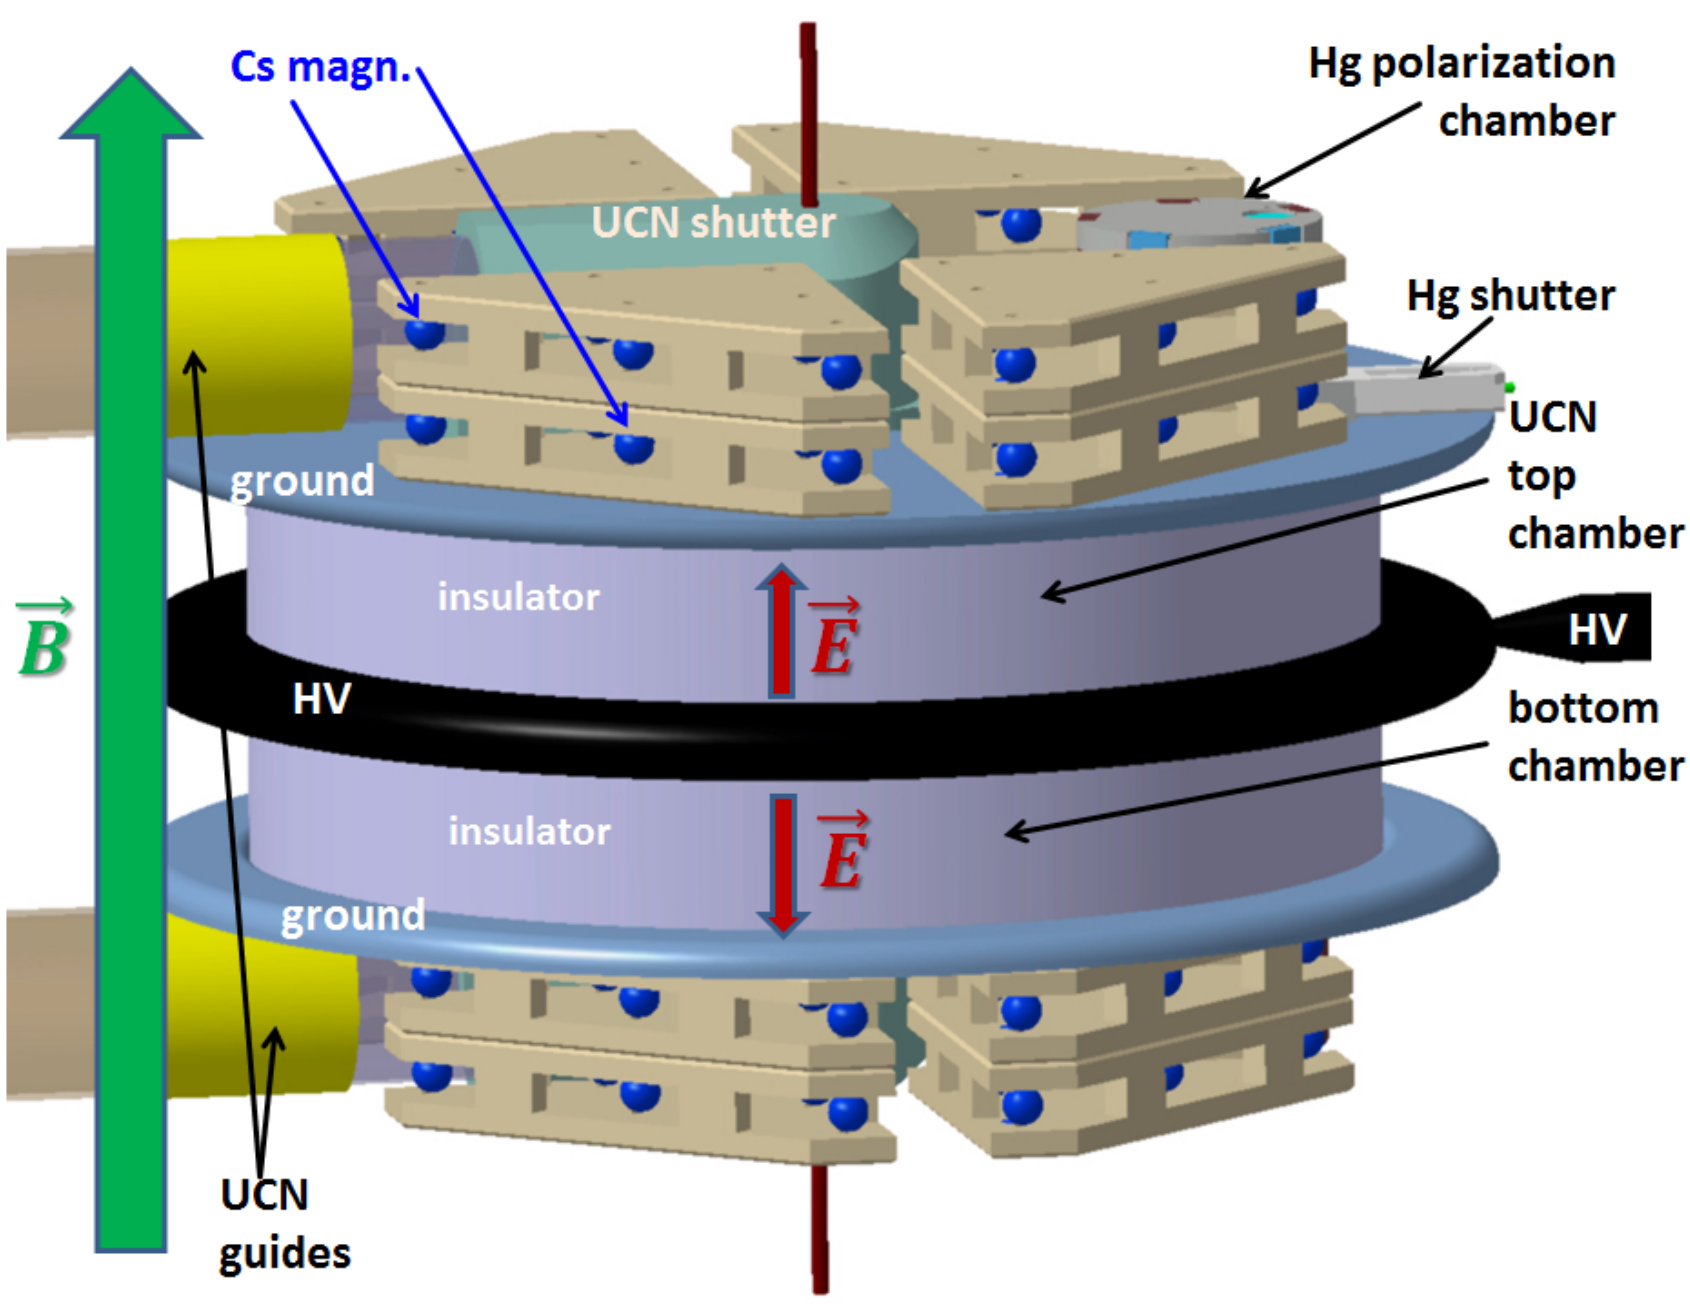
\includegraphics[width=\textwidth]{img/n2edm_chamber}
	\caption{Double chamber design \cite{Abel2018}.}
	\label{fig:precession_chamber}
\end{figure}

One can see that the precession chamber pictured in the Fig. \ref{fig:precession_chamber} features fields $\vec{E}$ and $\vec{B}$ that are codirectional in one chamber and contradirectional in another. In both chambers the neutron can be described with the Hamiltonian from Eq. \ref{eq:neutron_hamiltonian}. Let's take a look at its Larmor precession.

In the case of the \textbf{codirectional} fields we can write
\begin{equation}
	h\nu_{\uparrow \uparrow} = -2 \left( \mu_n B_{\uparrow \uparrow} + d_n E_{\uparrow \uparrow} \right).
	\label{eq:larmor_codirectional}
\end{equation}

If the fields are \textbf{contradirectional} we will get
\begin{equation}
	h\nu_{\uparrow \downarrow} = -2 \left( \mu_n B_{\uparrow \downarrow} - d_n E_{\uparrow \downarrow} \right).
	\label{eq:larmor_contradirectional}
\end{equation}

By combining Eq. \ref{eq:larmor_codirectional} and Eq. \ref{eq:larmor_contradirectional} we can express the neutron electric dipole moment $d_n$ through the fields $E$ and $B$, magnetic moment $\mu_n$ and Larmor frequencies $\nu_{\uparrow \uparrow}$ and $\nu_{\uparrow \downarrow}$ as
\begin{equation}
	d_n = \frac{h \left( \nu_{\uparrow \downarrow} - \nu_{\uparrow \uparrow} \right) - 2 \mu_n \left( B_{\uparrow \uparrow} - B_{\uparrow \downarrow} \right)}{2 \left( E_{\uparrow \uparrow} + E_{\uparrow \downarrow} \right)}.
\end{equation}

\textit{Why is the double chamber design important?} The idea of a double chamber pioneered \cite{Altarev1980} in 1980. The biggest improvement that it brings is the ability to measure the Larmor frequency for the codirectional and the contradirectional cases \textbf{simultaneously}. This feature allows to strongly reduce \cite{Abel2018} any time dependent systematic effects.

\textit{How does n2EDM look like schematically?} You can see it on the Fig. \ref{fig:n2edm_schema}.%
\begin{figure}[h]
	\centering
	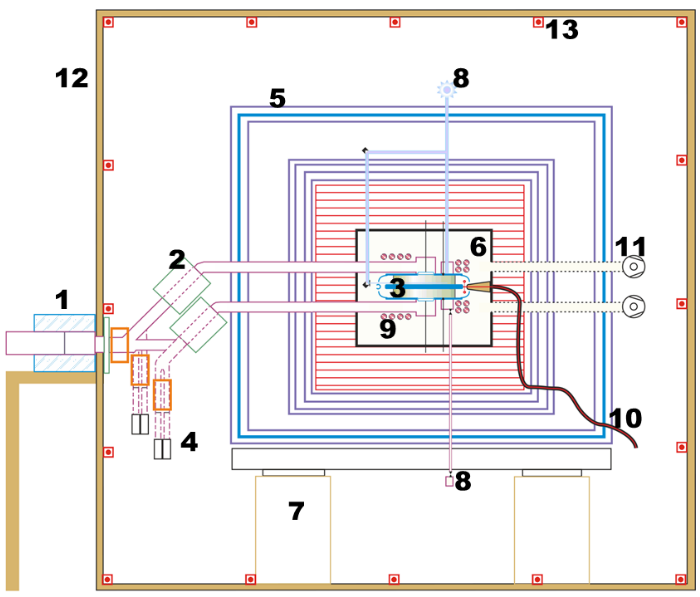
\includegraphics[width=.82\textwidth]{img/n2edm_schema}
	\caption{Schema of the experimental setup \cite{Abel2018}.}
	\label{fig:n2edm_schema}
\end{figure}

It features \cite{Abel2018} the following:
\begin{enumerate}
	\item A $5\ \text{T}$ superconductive polarizer magnet to align the spin of UCNs before they enter precession chambers
	\item Switches to control the filling and emptying of the UCN chambers
	\item Two precession chambers, portrayed in details on Fig. \ref{fig:precession_chamber}
	\item Four spin projection detectors --- for every chamber we count amount of neutrons with spins up and down
	\item Magnetically shielded room to protect the storage chambers and the vacuum vessel
	\item The vacuum vessel
	\item Four granite pillars supporting an $Al$ plate
	\item The $Hg$ magnetometer to measure the average magnetic fields
	\item The $Cs$ magnetometer to measure the gradients of the magnetic field
	\item A high voltage cable
	\item The molecular pumps generating vacuum in the vacuum vessel
	\item Insulation shell, thermally stabilized by air-conditioning (not shown)
	\item Surrounding field compensation (SFC) system is designed to actively minimise the magnetic perturbations of the environment
\end{enumerate}

\begin{figure}[h]
	\centering
	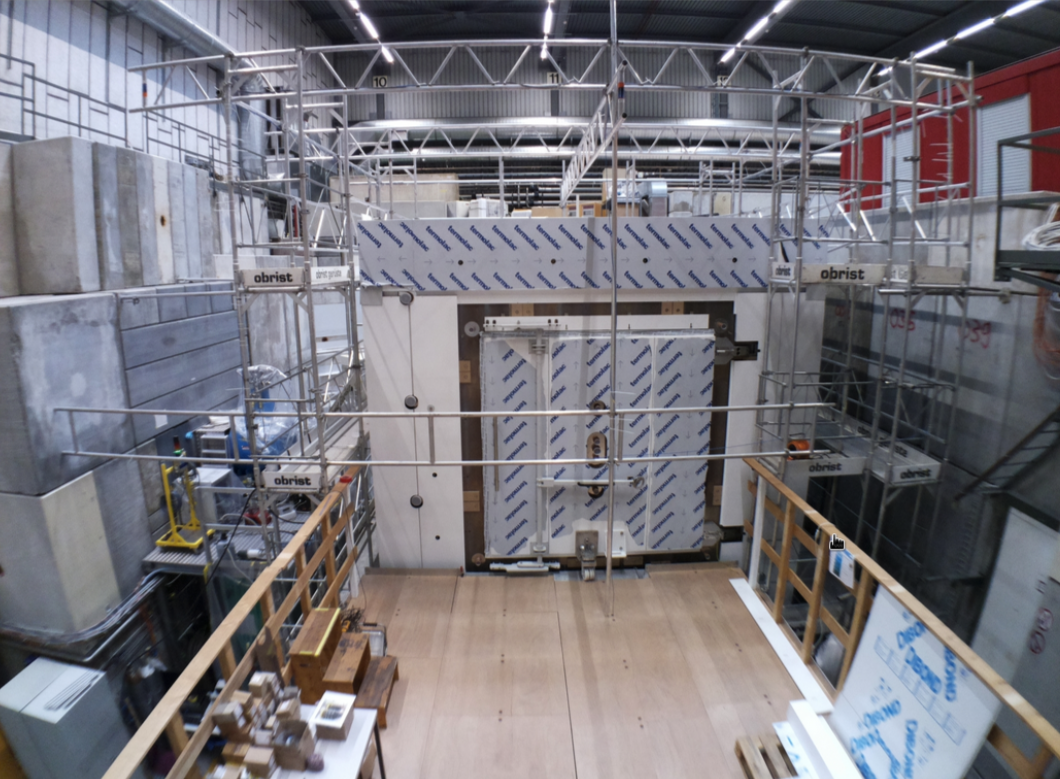
\includegraphics[width=.79\textwidth]{img/n2edm_photo}
	\caption{Recent photo of the n2EDM experiment.}
	\label{fig:n2edm_photo}
\end{figure}%